\RHpresentationHead{
  \documentclass[pdftex,unicode,xcolor=table]{beamer}
}

\mode<presentation> {
  \usetheme{Fedora}
  \setbeamertemplate{navigation symbols}{}
  \setbeamercovered{transparent=5}
}

\usepackage{beamerredhat}
\usepackage{etex}
\usepackage[utf8]{inputenc}
\usepackage{setspace,amsfonts,calc,upquote,hyperref,floatflt,graphicx}
\usepackage[table]{xcolor}
\usepackage{colortbl}
\usepackage[absolute,overlay]{textpos}\textposquirk


\title{Koschei}
\subtitle{Continuous integration in Koji}
\author{Author: \\
  \em{Mikolaj Izdebski}
  \tt{mizdebsk@redhat.com}}
\date{Date: \em{11 July 2014}}


\fancySectionOpens
%\fancyPartOpens

\begin{document}

\begin{rhbg}
  \begin{frame}
    \titlepage
    \begin{abstract}
Koschei is a service for scratch-rebuilding RPM packages in Fedora Koji
instance when their build-dependencies change or after some time elapse.

This presentation is about the problem Koschei is trying to solve, design decisions,
system structure, current status, plans for the nearest future and further
evolution possibilities.
    \end{abstract}
  \end{frame}
\end{rhbg}


\section{The problem}
\Large
\begin{frame}
  \frametitle{Where is the problem?}
  \begin{itemize}
  \item Buildability as a measure of software quality
    \begin{itemize}
      \item tests ran during build
    \end{itemize}
  \item Constantly growing number of packages
    \begin{itemize}
      \item software collections
    \end{itemize}
  \item People are unaware of FTBFS
    \begin{itemize}
      \item bugs are not seen until mass rebuild
      \item or worse, until there is critical bug to fix
    \end{itemize}
  \end{itemize}
\end{frame}

\begin{frame}
  \frametitle{Time elapse}
  Time elapse increases cost of fixing bugs
  \begin{itemize}
  \item People forget what they were working on
  \item More bugs appear
    \begin{itemize}
      \item Harder to discover where the real problem is
      \item Fixing means working in recursive, parallel mode
      \begin{itemize}
        \item to fix A you need to fix B first
        \item Koji repo regeneration
        \item ARM builders
      \end{itemize}
    \end{itemize}
  \end{itemize}
\end{frame}


\section{The solution}
\Large
\begin{frame}
  \frametitle{What can be done}
  Continuous integration
  \begin{itemize}
    \item continuous monitoring of package buildability
    \item helping maintainers to reason on FTBFS
  \end{itemize}
\end{frame}

\begin{frame}
  \frametitle{How?}
  \begin{itemize}
  \item Rebuild all packages from time to time
    \begin{itemize}
      \item weekly?
      \item too long delay
    \end{itemize}
  \item Rebuild important packages more often
    \begin{itemize}
      \item nightly?
      \item only a few packages can be rebuilt
    \end{itemize}
  \item Rebuild all rev deps after each update
    \begin{itemize}
      \item way too much resources needed
    \end{itemize}
  \item Middle ground solution?
  \end{itemize}
\end{frame}

\begin{frame}
  \frametitle{Where?}
  \begin{itemize}
  \item Options considered
    \begin{itemize}
      \item maintainers' machines
      \item Fedora Koji
      \item Copr
      \item cloud
    \end{itemize}
  \item The choice -- Fedora Koji
    \begin{itemize}
      \item existing, stable platform
      \item spare resources
      \item maintained by Fedora infrastructure
      \item no networking problems
      \item canonical build environment
    \end{itemize}
  \end{itemize}
\end{frame}


\Large
\begin{frame}
  \frametitle{Koschei}
  A tool for continuously scratch-rebuilding
  packages using Fedora build infrastructure -- Koji
\end{frame}

\large
\begin{frame}[fragile]
  \frametitle{Etymology}
\textbf{KO}ji \textbf{C}ontinuous \textbf{I}ntegration
\vspace{30 pt}
\begin{block}{Where did the name came from}
\begin{verbatim}
$ grep -xi ko*c*i /usr/share/dict/words
Koschei
\end{verbatim}
\end{block}
\end{frame}

\section{Design}
\begin{frame}
  \frametitle{The concept}
  \begin{itemize}
  \item A set of packages
  \item Reporting buildability
  \item Resource monitoring
  \item Rebuild prioritizing
  \end{itemize}
\end{frame}

\begin{frame}
  \frametitle{Priority}
  \begin{itemize}
    \item Time since last rebuild
    \item Dependency changes
    \begin{itemize}
      \item consider distances
    \end{itemize}
    \item Previous state
    \begin{itemize}
      \item prioritize failures
    \end{itemize}
    \item Importance
    \begin{itemize}
      \item aka static priority
    \end{itemize}
    \item Manual trigger
    \begin{itemize}
      \item aka dynamic priority
    \end{itemize}
    \item Plugins
  \end{itemize}
\end{frame}

\begin{frame}
  \frametitle{Database}
  \begin{itemize}
    \item Packages
    \begin{itemize}
      \item name
      \item priorities
    \end{itemize}
    \item Builds
    \begin{itemize}
      \item status
      \item Koji task ID
      \item time stamps
      \item logs
    \end{itemize}
    \item Repositories
    \begin{itemize}
      \item dependencies
    \end{itemize}
    \item Package groups
  \end{itemize}
\end{frame}

\begin{frame}[fragile]
  \frametitle{Architecture overview}
  \begin{center}
    \includegraphics[scale=0.25]{koschei.eps}
  \end{center}
\end{frame}

\begin{frame}
  \frametitle{Scheduler}
  \begin{itemize}
    \item Schedule package rebuilds
    \begin{itemize}
      \item priority scheduling
    \end{itemize}
    \item Request scratch builds on Koji
    \begin{itemize}
      \item from existing SRPM
      \item very low priority
      \item needs Koji certificate
    \end{itemize}
    \item Conditions
    \begin{itemize}
      \item build group is installable
      \item package monitoring is enabled
      \item package is not blocked
      \item build dependencies are resolvable
      \item priority is high enough
      \item Koji load is low enough
    \end{itemize}
  \end{itemize}
\end{frame}

\begin{frame}
  \frametitle{Koji load}
  \begin{itemize}
    \item Task load
    \begin{itemize}
      \item default channel
      \item handling of disabled hosts
      \item handling of not ready hosts
      \item per-architecture load
      \item current threshold: 50 \%
    \end{itemize}
    \item Number of Koschei tasks
    \begin{itemize}
      \item current threshold: 30 tasks
    \end{itemize}
  \end{itemize}
\end{frame}

\begin{frame}
  \frametitle{Polling}
  \begin{itemize}
    \item Koji
    \begin{itemize}
      \item scratch build statuses
      \item real builds
      \item check blocked packages
    \end{itemize}
    \item pkgdb2
    \begin{itemize}
      \item user ACLs
    \end{itemize}
  \end{itemize}
\end{frame}

\begin{frame}
  \frametitle{Resolver}
  \begin{itemize}
    \item Analyze dependency changes
    \begin{itemize}
      \item download latest repodata from kojipkgs
      \item resolve build group
      \item resolve package build-dependencies
      \item hawkey
    \end{itemize}
    \item Update priorities
    \begin{itemize}
      \item increase priority on dependency change
      \item reset priority on build success
    \end{itemize}
  \end{itemize}
\end{frame}

\begin{frame}
  \frametitle{Watcher}
  \begin{itemize}
    \item \tt{buildsys.task.state.change}
    \item \tt{buildsys.repo.done}
    \item \tt{buildsys.build.tag}
    \item \tt{pkgdb.*}
  \end{itemize}
\end{frame}

\begin{frame}
  \frametitle{Web frontend}
  \begin{itemize}
    \item OpenID login
    \item package list view
    \item package groups
    \item build details
    \item documentation
    \item adding packages
  \end{itemize}
\end{frame}

\section{Implementation}
\begin{frame}
  \frametitle{Implementation}
  \begin{itemize}
    \item Python
    \item PostgreSQL
    \item SQLAlchemy, Alembic
    \item Modularity
    \item hawkey
    \item systemd
  \end{itemize}
\end{frame}

\begin{frame}[fragile]
  \begin{center}
    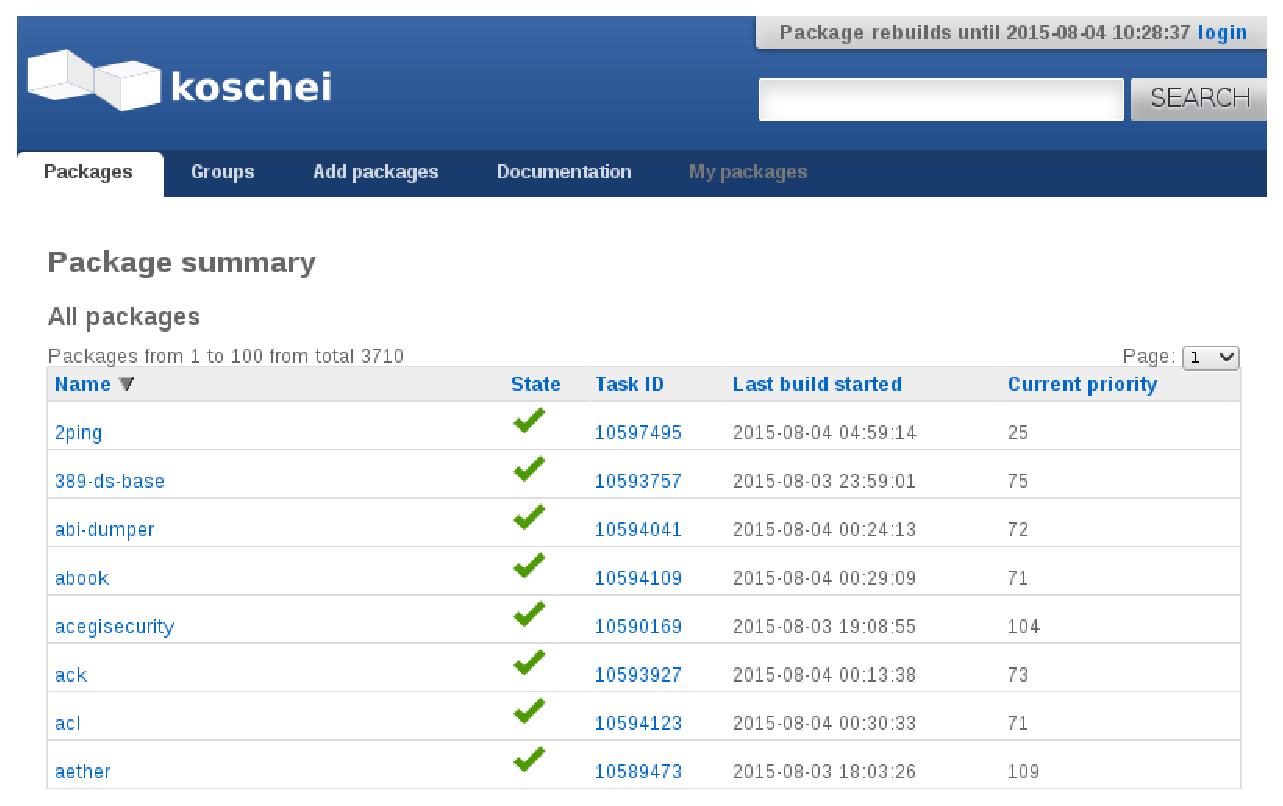
\includegraphics[scale=0.48]{koschei-frontend-1.eps}
  \end{center}
\end{frame}

\begin{frame}[fragile]
  \begin{center}
    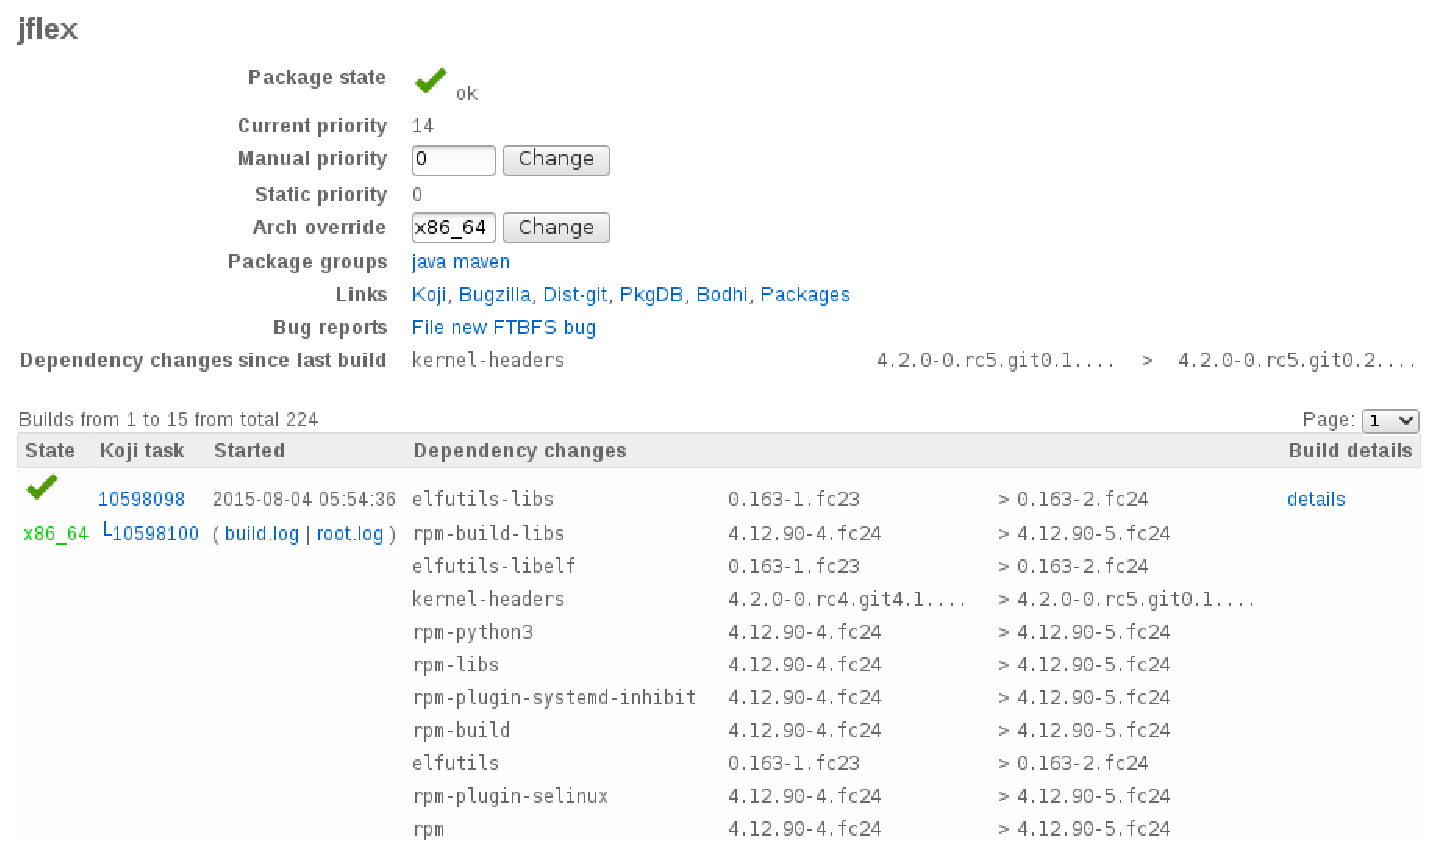
\includegraphics[scale=0.48]{koschei-frontend-2.eps}
  \end{center}
\end{frame}

\begin{frame}[fragile]
  \begin{center}
    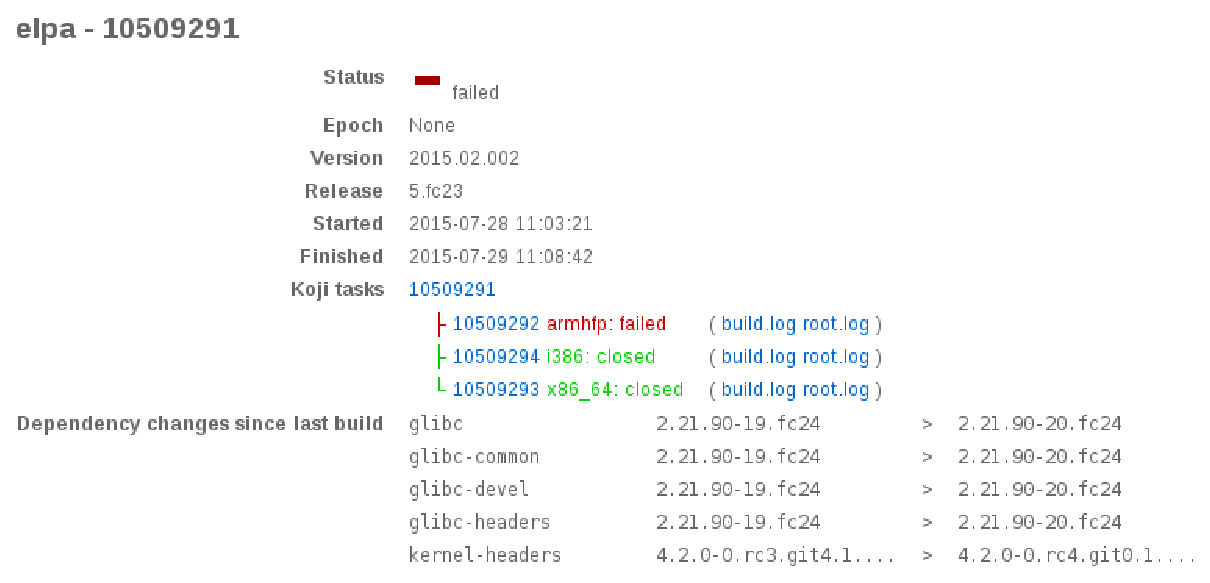
\includegraphics[scale=0.48]{koschei-frontend-3.eps}
  \end{center}
\end{frame}

\begin{frame}
  \frametitle{Current state}
  \begin{itemize}
    \item code at Github
    \item available in Fedora and EPEL 7
    \item running at Fedora infrastructure
  \end{itemize}
\end{frame}

\section{Future}
\begin{frame}
  \frametitle{TODO}
  \begin{itemize}
    \item pkgdb2 integration
    \item UI improvements
    \item RPC / CLI interface
    \item immediate scratch build purging
    \item more fedmsg events
    \item non-rawhide tags?
    \item automatic bug filing?
  \end{itemize}
\end{frame}

\begin{frame}
  \frametitle{Links}
  \begin{itemize}
    \item Production instance
    \begin{itemize}
      \item \url{https://apps.fedoraproject.org/koschei}
    \end{itemize}
    \item Documentation
    \begin{itemize}
      \item \url{https://fedoraproject.org/wiki/Koschei}
    \end{itemize}
    \item Code repository
    \begin{itemize}
      \item \url{https://github.com/msimacek/koschei}
    \end{itemize}
  \end{itemize}
\end{frame}


\mode<presentation> {
  \Rhbg{\frame{\theend}}
}

\end{document}
